\appendix 
%\appendixpage
\chapter{OSI Model}
\label{osi}
  \begin{center}
  \begin{tabular}{|lc|}
  \hline
  7: &
  Application Layer \\
  & (e.g. DNS, DHCP) \\
  \hline
  6: &
  Presentation Layer \\
  & (e.g. telnet) \\ 
  \hline
  5: &
  Session Layer \\
  & (e.g. RPC) \\
  \hline
  4: &
  Transport Layer \\
  & (e.g. TCP, UDP) \\
  \hline
  3: &
  Network Layer \\
  & (e.g. IPv4, IPv6) \\
  \hline  
  2: &
  Data Link Layer \\
  & (e.g. MAC) \\ 
  \hline  
  1: &
  Physical Layer \\
  & (e.g. Ethernet, Wi-Fi) \\
  \hline
\end{tabular}
\end{center}

The seven layer OSI model is a logical grouping of the types of protocols found
in computer networks. Each layer is dependent only on the layer directly below
it. 

The TCP/IP model is a similar, but simpler model of networking.

\chapter{Packets}
Images created with http://interactive.blockdiag.com/packetdiag/

\chapter{Netkit}
\section{Screenshot of Netkit running}
\begin{center}
	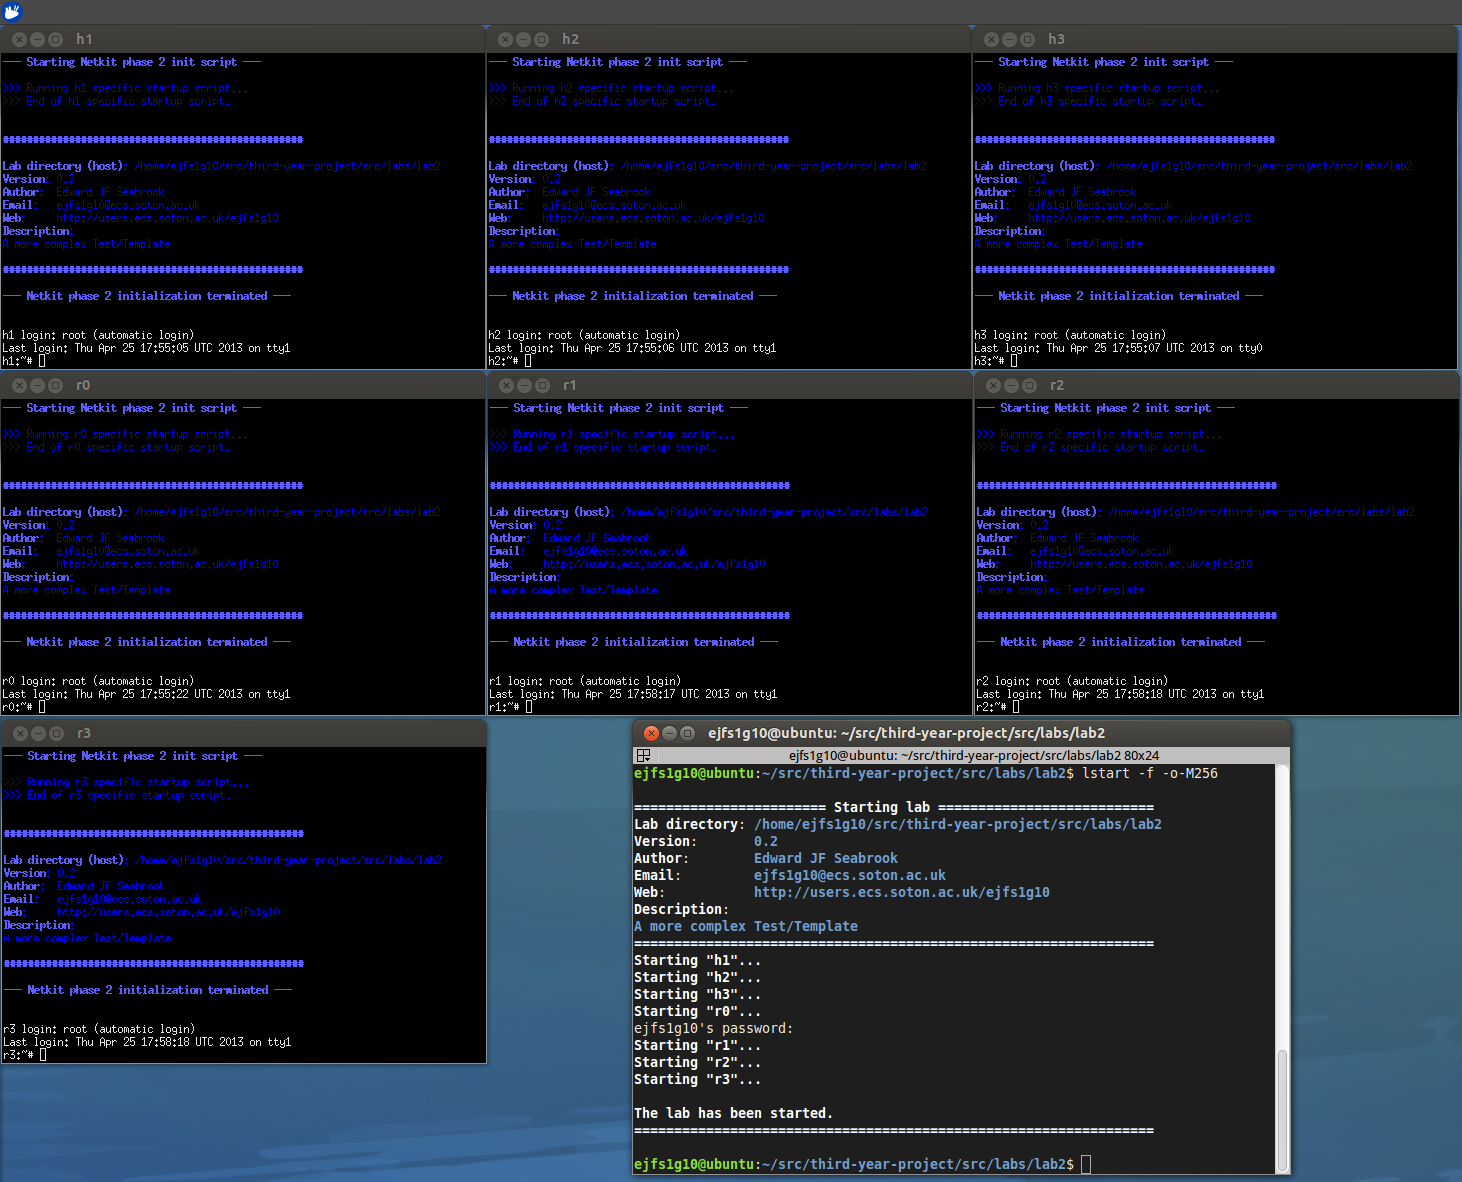
\includegraphics[width=\linewidth]{../Diagrams/Netkit/NetkitScreenshot.png}
\end{center}

\chapter{Github Stats}
\label{GithubStats}

\section{Github Commit Graph}
\begin{center}
	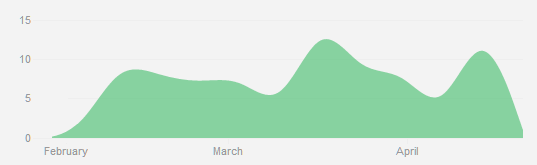
\includegraphics[width=\linewidth]{../Diagrams/Stats/GitHubCommitGraph.png}
\end{center}

\section{Github Punchcard}
\begin{center}
	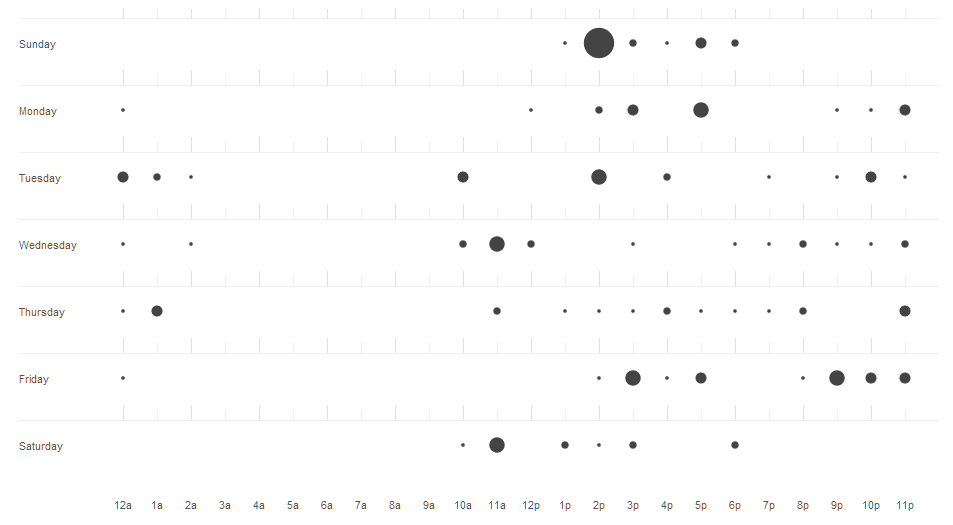
\includegraphics[width=\linewidth]{../Diagrams/Stats/GitHubPunchCard.png}
\end{center}

\chapter{Alix2d3}
As the project progressed it became clear that they Alix2d3s were not as useful
as was originaly believed, thanks to discovery of the briliant software package
Netkit. I did however undertake testing on the Alix2d3s. If someone wished to
repeat my experimentation, the following guides would be helpful. 

\section{Installation Guide}

 This guide\cite{germanGuide} offered a comprehensive list of steps that need to
 be taken to install Ubuntu Linux on a PC Engines alix2d3\cite{alix2d3}.  The article is
 written in German but using Google translate I was able to follow it as it is
 mainly a list of shell commands.

 The process begins with installing the compact flash card as a device on an
 existing Ubuntu desktop PC\@. Next the card is partitioned using \texttt{fdisk},
 the card is then formatted as ext2 (a Linux file system type) using
 \texttt{mk2fs}. The card is then mounted in the file system, using
 \texttt{mount} and a small installation of Linux is copied to the card using
 \texttt{debootstrap} to provide a base system.

 Several settings and devices are linked to the flash cards mount point and
 \texttt{chroot} is used to simulate booting into the new install. The required
 configuration files are edited (e.g.\@ network interface settings) and essential
 software packages (such as \texttt{Vim}, \texttt{SSH}, \texttt{sudo}, and
 \texttt{APT}) are installed. A boot loader such as \texttt{GRUB} is also
 installed and configured.

 Next, the flash card is safely removed, and  inserted into the alix2d3. The
 alix2d3 is then powered on. Using a USB to Null Model cable connecting a PC to
 the alix2d3's serial port, a terminal connection can be established using {\bf
 cu}. I had a few problems using this device (\texttt{ttyUSB0}) but I was able to
 fix this problem using \texttt{chown}. This terminal connection can be used to
 aid the boot process and ensure that there are no Magic ELF errors. Once the
 alix2d3 is up and running it is possible to disconnect the serial cable and
 access it over \texttt{SSH} alone.

 \section{Quagga Installation Guide}

 \subsection{Normal Installation}
This is a procedure that has  turned out to be far more difficult that anticipated.

First of all, need to ensure that all the dependencies are present. The easiest
way I have found to do this is to use:

sudo apt-get build-dep quagga

This should fetch all the packages that quagga depends on. I see no reason to
build these from source, since I shall not be modifying them.

It seems that a package called libtool is also needed to ensure installation works.
Not certain this is needed.

\ libreadline also seems to be an issue (mainly with vtysh):

\texttt{sudo apt-get install lib32readline6}

Next it should be possible to run \texttt{\@./bootstrap}. As far as I know this
produces (among other things) the configure script.

Next run the configure script. This [wiki][wiki] suggests that it is best to
move the folders using:

\texttt{sudo \@./configure --sysconfdir=/usr/local/quagga --localstatedir=/usr/local/quagga}

The configure script will prompt you to create a user called quagga. Do this by:

sudo adduser quagga
sudo mkdir /usr/local/quagga
sudo chown quagga:quagga /usr/local/quagga

It is now time to run make. See the crosscompiling document for more
information about this. Previously I had issues with zebra making, to fix this
manually editing the Makefile in \@./zebra by adding -lcap to LIBS\@. This doesn't
seem to be a problem with the latest source.

Run sudo make install. This should install everything, and the daemons
should have installed themselves to /usr/local/sbin.

Now a little bit of configuration is required. \texttt{cd /usr/local/quagga}.
Either make a real config file for the daemon, or just create a file containing ``password test''.


You should now be able to run sudo ospf6d. If you can't, try ldconfig.


[wiki]: http://wiki.nil.com/Installing\_and\_running\_Quagga

\subsection{Cross Compilation}

Since Alix2d3s are very slow, a build of Quagga can be incredibly slow. The make parts
alone can take around 15 minutes. (I actually found that XORP had an even slower
compile time, in the order of hours) 

To over come this issue it is possible to compile the source code on a much
faster machine (e.g.\@ desktop pc) and copy it across. 

Since modern machines use a 64bit architecture rather than 32bit like the
Alix2d3s, the compiler must be set up correctly. Adding the cflag ``-m32'' should
suffice, however to be on the safe side, ``-m32 -march=i386'' can be used. 

This should be done by appending '--with-clfags=``-m32 -march=i386i''' to \@./configure.

I initially had problems with this compilation. I resolved the issues by going
back to basics and trying to compile a simple helloworld program for the Alix.
Turns out I was missing ``gcc-multilib''. This can be installed with apt.

\chapter{vtysh}
\label{vtysh}

Commands are added using DEFUN and install.

I added the commands:
\begin{itemize}
  \item show ipv6 ospf6 prefix aggregated
  \item show ipv6 ospf6 prefix allocated 
  \item show ipv6 ospf6 prefix assigned X

  \item enable $>$ configure terminal $>$ ipv6 allocate-prefix X:X::X:X/M
  \item enable $>$ configure terminal $>$ no ipv6 allocate-prefix X:X::X:X/M
\end{itemize}
